\graphicspath{{images/agreement/}}

\section{Договоры}
Для перехода в раздел необходимо нажать ссылку \quotes{Договоры} на главной панели, ссылка выделена на рисунке ~\ref{agreement:agreement_section}.
\begin{figure}[H]
	\center{
\includegraphics[width=1\linewidth]{agreement_section.png}}
	\caption{Ссылка для перехода в раздел \quotes{Договоры}}
	\label{agreement:agreement_section}
\end{figure}
Платформа позволяет реализовать следующий сценарий: на Платформе создаются университеты, администраторы добавляют курсы, которые привязываются к разработавшему их вузу. В дальнейшем университеты могут заключать между собой договоры на покупку права обучать студентов одного университета на курсах другого в течение периода времени, установленного договором. В этом случае университет, предоставляющий свои курсы называется вузом"=разработчиком (поставщиком), университет, осуществляющий покупку, "--- вузом-потребителем (потребителем). Один и тот же университет может выступать как поставщик в одних договорах и как потребитель в других.\\
Университет не может выступать в роли поставщика, если у него установлен флаг \quotes{Является только потребителем} (флаг устанавливается \quotes{Суперпользователем}).\\
Помимо перечисленного вуз может быть потребителем и поставщиком в рамках одного договора, то есть разрешено создание договоров с самим собой.

Раздел \quotes{Договоры} предоставляет средства для организации этапов описанного выше сценария.

Краткое описание состава раздела:
\begin{itemize}
	\item \textbf{Функции поставщика}
	\begin{itemize}
		\item \textbf{Договоры на предоставление услуг.} Подраздел выводит информацию о договорах, в которых данный университет является поставщиком. Из этого подраздела осуществляется переход к подразделам:
		\begin{itemize}
			\item \textbf{Просмотр информации о договоре.} Предоставляет подробную информацию о договоре. \\
			В этом разделе можно произвести попытку \textbf{удаления договора}.
			\item \textbf{Редактирование договора.} Предоставляет поставщику возможность редактирования созданного договора
		\end{itemize}
		\item \textbf{Платежи.} Платежи слушателей курса за прохождение курса.
		\item \textbf{Заявки на зачисление.} Вузы"=потребители могут подавать заявки на зачисление своих студентов, перечисленных в заявке, на курсы вуза"=разработчика. В этом подразделе выводится информация о заявках, поступивших данному университету, как поставщику.  Из этого подраздела осуществляется переход к подразделу:
		\begin{itemize}
			\item \textbf{Просмотр информации и управление статусом заявки.} Предоставляет подробную информацию о заявке. В этом подразделе поставщик может принять или отклонить поступившую заявку.
		\end{itemize}
		\item \textbf{Заявки на изменение режима прохождения сессии курса.} Для сессии курса может существовать несколько режимов прохождения (подробнее см. раздел \quotes{Курсы}), вуз"=потребитель может подавать заявки на изменение режима прохождения сессии для группы своих студентов из числа зачисленных, которая указана в заявке. В этом подразделе выводится информация о заявках на изменение режима прохождения сессии, поступивших данному университету, как поставщику. Из этого подраздела осуществляется переход к подразделу:
		\begin{itemize}
			\item \textbf{Просмотр информации и управление статусом заявки.} Предоставляет подробную информацию о заявке. В этом подразделе поставщик может принять или отклонить поступившую заявку.
		\end{itemize}
		\item \textbf{Добавить договор.} Подраздел предоставляет поставщику возможность создания договора.
	\end{itemize}
	
	\item \textbf{Функции потребителя}
	\begin{itemize}
		\item \textbf{Договоры на получение услуг.} Подраздел выводит информацию о договорах, в которых данный университет является потребителем. Из этого подраздела осуществляется переход к подразделу
		\begin{itemize}
			\item \textbf{Просмотр информации о договоре.} Предоставляет подробную информацию о договоре.
		\end{itemize}
	\end{itemize}
\end{itemize}

Навигация по компонентам раздела осуществляется с помощью левой панели вспомогательного меню, структура которого соответствует описанному выше составу раздела (см. рис.\ref{agreement:menu})
	
	\begin{figure}[H]
	\center{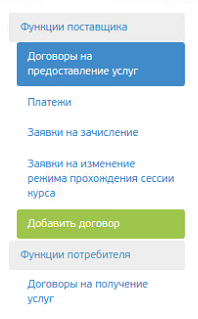
\includegraphics[width=0.4\linewidth]{menu.png}}
	\caption{Внешний вид меню навигации раздела \quotes{Договоры}}
	\label{agreement:menu}
	\end{figure}

\subsection{Роли и операции}
Раздел доступен пользователям, имеющим следующие роли:	
	\begin{itemize}
		\item Администратор вуза, если вуз является поставщиком и потребителем::
		\begin{itemize}
			\item просмотр списка договоров на предоставление услуг;
			\item просмотр подробной информации о договорах на предоставление услуг;
			\item удаление договоров на предоставление услуг;
			\item редактирование договоров на предоставление услуг;
			\item просмотр платежей;
			\item просмотр заявок на зачисление и управление статусом заявок;
			\item просмотр заявок на изменение режима прохождения сессий и управление статусом заявок;
			\item создание договоров на предоставление услуг;
			\item просмотр списка договор на получение услуг (выводятся только договоры в статусе \quotes{Действует}); 
			\item просмотр подробной информации о действующих договорах на получение услуг.
		\end{itemize}
		\item Администратор вуза, если вуз является только потребителем::
		\begin{itemize}
			\item просмотр списка договор на получение услуг (выводятся только договоры в статусе \quotes{Действует}); 
			\item просмотр подробной информации о действующих договорах на получение услуг.
		\end{itemize}
		\item Автор курса:
		\begin{itemize}
			\item просмотр списка договоров на предоставление услуг (притом выводится информация только по тем договорам, в которых участвуют курсы, автором которых является данный пользователь), иконка редактирования для перехода в подраздел \quotes{Редактирование договора} для этой роли скрывается;
			\item просмотр подробной информации о договорах на предоставление услуг(имеются в виду те договоры, в которых участвуют курсы, автором которых является данный пользователь), подробная информация выводится только по тем курсам, автором которых является данный пользователь.
		\end{itemize}						
	\end{itemize} 
	
	\subsection{Договоры на предоставление услуг}\label{agreement:provider_agreements_section}
При выборе в главном меню пункта \quotes{Договоры} осуществляется переход в подраздел \quotes{Договоры на предоставление услуг}, если роль пользователя позволяет просматривать этот подраздел.
Подраздел предоставляет информацию о договорах, в которых данный вуз выступает в роли поставщика. Информация представлена в виде таблицы, строки которой соответствуют договорам. Внешний вид раздела  приведён на рисунке~\ref{agreement:provider_agreements}
	
	\begin{figure}[H]
	\center{\includegraphics[width=1\linewidth]{provider_agreements.png}}
	\caption{Внешний вид подраздела \quotes{Просмотр договоров на предоставление услуг}}
	\label{agreement:provider_agreements}
	\end{figure}
	
\textbf{Перечень столбцов таблицы:}
\begin{itemize}
	\item \textbf{Номер.} Номер договора является ссылкой, по нажатию осуществляется переход к подразделу \quotes{Просмотр подробной информации о договоре}.
	\item \textbf{Вуз"=потребитель.} Аббревиатура вуза"=потребителя, с которым заключен данный договор, является ссылкой, по нажатию осуществляется переход на станицу университета на сайте.
	\item \textbf{Дата начала.} Дата начала договора.
	\item \textbf{Дата окончания.} Дата окончания договора.
	\item \textbf{Статус.} Статус договора принимает одно из трех возможных значений: \quotes{Черновик},  \quotes{Действует},  \quotes{Не действует}. Создание заявок на зачисление на стороне потребителя возможно только по действующему договору. Договоры, имеющие статус  \quotes{Черновик} и \quotes{Не действует} не показываются потребителям в соответствующем разделе \quotes{Договоры на получение услуг}.
	\item \textbf{Количество студентов.} При создании/редактировании договора можно указывать максимальное количество студентов для каждого курса, которые могут быть зачислены по данному договору. Количество студентов "--- суммарное максимальное количество студентов по всем курсам, указанным в договоре, может быть не заполнено.
	\item \textbf{Зачислено.} Фактическое суммарное количество зачисленных студентов по данному договору на текущий момент.
	\item \textbf{Иконка редактирования.} По нажатию  \vcenteredinclude[height=17px]{edit_icon.png} осуществляется переход в подраздел \quotes{Редактирование договора}, скрывается в случае, если роль пользователя не позволяет редактировать договоры.
\end{itemize}

\subsubsection{Элементы управления}
Помимо общих элементов управления табличными данными, описанных в подразделе~\ref{sec:datatables}, на странице раздела присутствует 
иконка \quotes{Справка} \vcenteredinclude[height=25px]{table_help.png}, которая выводит справочную информацию о таблице. 
При нажатии появляется всплывающее окно, в котором описан принцип подсветки фона строк таблицы: 
цвет фона строки отличается в зависимости от наличия и статуса заявок на зачисление студентов или изменения режима прохождения сессии по договору, которому соответствует  данная строка (см. рис.~\ref{agreement:table_help_legend}), возможны три варианта:
\begin{itemize}
	\item есть нерассмотренные заявки;
	\item все заявки одобрены;
	\item заявок нет.
\end{itemize}	
\begin{figure}[H]
\center{\includegraphics[width=1\linewidth]{table_help_legend.png}}
\caption{Всплывающее окно с подсказкой}
\label{agreement:table_help_legend}
\end{figure}	

Форма фильтрации в данном подразделе позволяет задавать следующие параметры:
\begin{itemize}
	\item университет - позволяет выбрать одного или нескольких вузов-потребителей, принципы работы с полями такого типа описаны в подразделе ~\ref{widget:autocomplete_with_multiselect};
	\item статус договора;
	\item дата начала договора от (принципы работы с полями такого типа описаны в подразделе ~\ref{widget:date_time_picker});
	\item дата начала договора до (принципы работы с полями такого типа описаны в подразделе ~\ref{widget:date_time_picker});
	\item дата окончания договора от (принципы работы с полями такого типа описаны в подразделе ~\ref{widget:date_time_picker});
	\item дата окончания договора до (принципы работы с полями такого типа описаны в подразделе ~\ref{widget:date_time_picker});
	\item заявки - позволяет отфильтровать договоры в соответствии с наличием и статусом заявок, принципы работы с полями такого типа описаны в подразделе ~\ref{widget:autocomplete_with_multiselect};
\end{itemize}

\subsection{Договоры на получение услуг}
Переход в данный подраздел осуществляется по выбору соответствующего пункта вспомогательного меню на панели, расположенной слева (см. рис. ~\ref{agreement:menu}).

Данный подраздел предоставляет информацию о договорах, в которых данный вуз является потребителем, причем отображается только информация по договорам в статусе \quotes{Действует}.

Содержание подраздела, возможные действия и реакции полностью аналогичны описанным в подразделе~\ref{agreement:provider_agreements_section} за исключением двух моментов:
\begin{itemize}
	\item В таблице, содержащей информацию о договорах отсутствует колонка с иконкой для переход к подразделу \quotes{Редактирование договора}, так как администратор вуза, который является только потребителем, не имеет права на редактирование договоров.
	\item В таблице, содержащей информацию о договорах отсутствует колонка \quotes{Статус}, так как в данном разделе выводится информация только о действующих договорах. Договоры в статусе \quotes{Черновик} и \quotes{Не действует}, заключенные с данным вузом"=потребителем, видны только из кабинетов поставщиков, заключивших эти договоры.
	\item В таблице, содержащей информацию о договорах, вместо колонки \quotes{Вуз-потребитель} добавлена колонка \quotes{Вуз-разработчик}, содержащая аббревиатуру вуза-разработчика в договоре, является ссылкой на страницу университета на сайте.
\end{itemize}


\subsection{Просмотр подробной информации по договору}
Позволяет просмотреть подробную  информацию по интересующему договору. Информацию по заключенному договору доступна для просмотра как поставщику, так и потребителю, однако, для последнего она выводится в ограниченном виде.

Администратор вуза может просматривать полную информацию по всем договорам, в которых вуз выступает в роли поставщика и ограниченную информацию по действующим договорам, в которых вуз является поставщиком.

Автор курса может просматривать ограниченную информацию о договорах, в которых фигурируют курсы, автором которых он является.

Перейти в раздел можно, нажав на номер договора в таблице в разделе \quotes{Просмотр договоров на предоставление услуг} (просмотр в роли поставщика, автора курсов), или в разделе \quotes{Просмотр договоров на получение услуг} (просмотр в роли потребителя). \\
Внешний вид подраздела с полной информацией приведён на рисунке~\ref{agreement:detail}
	
	\begin{figure}[H]
	\center{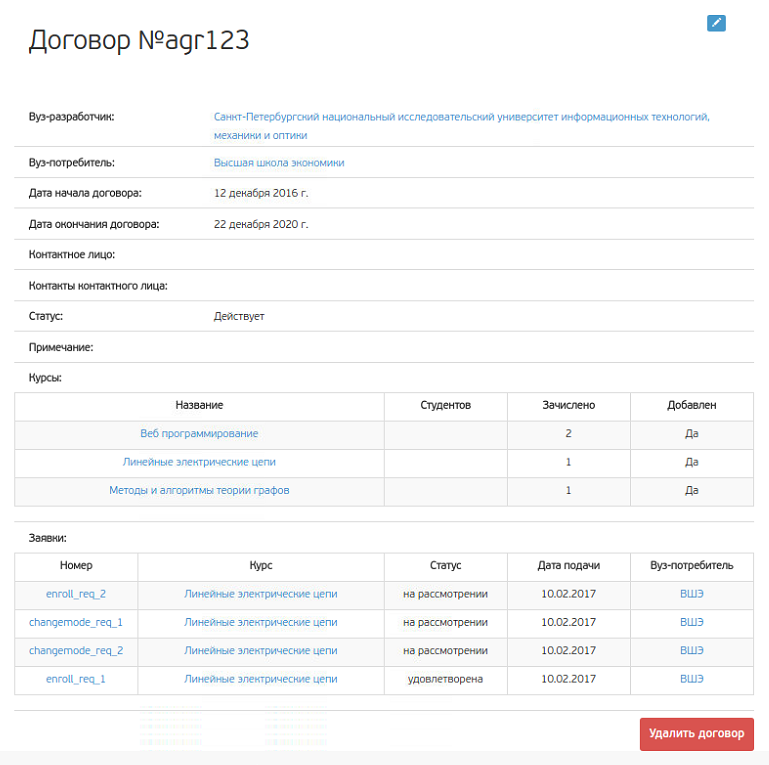
\includegraphics[width=1\linewidth]{detailview.png}}
	\caption{Просмотр подробной информации о договоре: полный набор полей и элементов управления}
	\label{agreement:detail}
	\end{figure}

Набор доступных для просмотра полей отличается в зависимости от роли пользователя и того, поставщиком или потребителем в конкретном договоре выступает вуз, из кабинета которого осуществляется просмотр.
\begin{itemize}
	\item При просмотре подробной информации по договорам на предоставление услуг:
	\begin{itemize}
		\item администратору вуза доступны все перечисленные ниже поля;
		\item автору курсов доступны только поля, выделенные жирным шрифтом;
	\end{itemize}
	\item При просмотре подробной информации по договорам на получение услуг администратору вуза доступны только поля, выделенные жирным шрифтом.
\end{itemize}
Поля:
\begin{itemize}
	\item \textbf{Номер договора.} Указан в заголовке.
	\item \textbf{Вуз разработчик.} Название вуза, который выполняет роль поставщика в данном договоре. Является ссылкой, по нажатию осуществляется переход на страницу университета на сайте.
	\item \textbf{Вуз потребитель.} Название вуза, который выполняет роль потребителя в данном договоре. Является ссылкой, по нажатию осуществляется переход на страницу университета на сайте.
	\item \textbf{Дата начала договора.}
	\item \textbf{Дата окончания договора.}
	\item \textbf{Контактное лицо.} Контактное лицо со стороны вуза"=потребителя для связи по данному договору.
	\item \textbf{Контакты контактного лица.} Контакты (e"=mail, номер телефона, др.) контактного лица со стороны вуза"=потребителя для связи по данному договору.
	\item Статус договора принимает одно из трех возможных значений: \quotes{Черновик},  \quotes{Действует},  \quotes{Не действует}. Создание заявок на зачисление на стороне потребителя возможно только по действующему договору. Договоры, имеющие статус  \quotes{Черновик} и \quotes{Не действует} не показываются потребителям в соответствующем разделе \quotes{Договоры на получение услуг}.
	\item Примечание. Любое примечание поставщика.
	\item \textbf{Курсы.} Информация о курсах, связанных с данным договором, представлена в виде таблицы, строка таблицы соответствует курсу. \\
	Курс является связанным с договором в нескольких случаях:
	\begin{itemize}
		\item курс добавлен к данному договору поставщиком в форме создания/редактирования договора;
		\item по данному курсу имеются заявки (на зачисление/изменение режима прохождения сессии) в любом статусе, в которых указан данный договор;
		\item на курс когда-либо были зачислены студенты с указанием данного договора;
	\end{itemize}
	При просмотре в роли \quotes{автор курса} показываются только те курсы, автором которых является данный пользователь.\\
	Таблица курсов содержит следующие столбцы:
	\begin{itemize}
		\item \textbf{Название.} Название курса;
		\item \textbf{Студентов.} Максимальное количество студентов, которое можно зачислить по данному договору. Указывается поставщиком при создании/редактировании договора, может быть не заполнено;
		\item\textbf{ Зачислено.} Фактическое количество студентов, зачисленных по данному договору на текущий момент;
		\item \textbf{Добавлен.} Флаг, показывающий добавлен ли конкретный курс поставщиком в договор;
	\end{itemize}	
	\item Заявки. Информация о заявках на зачисление студентов по данному договору, если таковые имеются, представлена в виде таблицы.\\
	Таблица заявок содержит следующие столбцы:
	\begin{itemize}
		\item Номер. Номер заявки;
		\item Курс. Курс, на который подана заявка;
		\item Статус. Статус заявки;
		\item Дата подачи. Дата подачи заявки;
		\item Вуз"=потребитель. Вуз, со стороны которого была подана заявка.
	\end{itemize}
\end{itemize}

\subsubsection{Элементы управления}
В данном разделе имеются следующие элементы управления, которые видны при просмотре подробной информации по договорам на предоставление услуг, для пользователей роли \quotes{Администратор вуза}:
\begin{itemize}
	\item иконка \vcenteredinclude[width=0.1\linewidth]{edit_icon.png}, нажатие на иконку переводит пользователя в подраздел \quotes{Редактирование договора};
	\item кнопка \quotes{Удалить договор}, по нажатию осуществляется попытка удаление договора.
\end{itemize}

\subsection{Удаление договора}
Для того, чтобы произвести попытку удаления договора, необходимо нажать кнопку \quotes{Удалить договор} в нижней части страницы раздела \quotes{Просмотр подробной информации по договору} (см. рис.~\ref{agreement:detail}), которая доступна при просмотре подробной информации по договору на предоставление услуг пользователям роли \quotes{Администратор вуза}. Далее возможны два варианта: либо договор можно удалить, либо нет.\\
Договор нельзя удалить в следующих случаях:
\begin{itemize}
	\item имеются заявки в любом статусе с указанием этого договора;
	\item по договору когда-либо были зачислены студенты.
\end{itemize} 
Если договор можно удалить, то по нажатию кнопки \quotes{Удалить} будет показано модальное окно с вопросом о подтверждении удаления см. рис.~\ref{agreement:delete_yes}.

\begin{figure}[H]
	\center{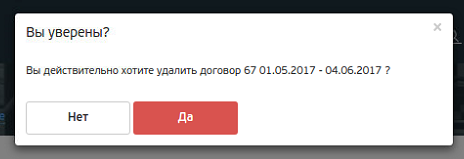
\includegraphics[width=1\linewidth]{delete_yes.png}}
	\caption{Окно подтверждения удаления договора}
	\label{agreement:delete_yes}
\end{figure}

Прервать удаление можно, нажав кнопку \quotes{Нет} или "X" в верхнем правом углу модального окна, или, нажав за пределы окна. Если прервать операцию удаления, модальное окно закроется, пользователь останется в разделе \quotes{Просмотр подробной информации по договору}.\\
Подтвердить удаление можно, нажав кнопку \quotes{Да} модального окна, тогда произойдет удаление договора, пользователь будет перенаправлен в подраздел \quotes{Договоры на предоставление услуг}. \\ \\
Если договор нельзя удалить, то по нажатию кнопки \quotes{Удалить} будет показано модальное окно с информацией, по каким причинам этого нельзя сделать см. рис.~\ref{agreement:delete_no}.

\begin{figure}[H]
	\center{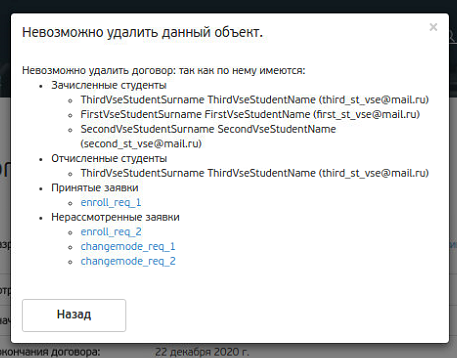
\includegraphics[width=1\linewidth]{delete_no.png}}
	\caption{Окно с информацией о причинах невозможности удаления договора}
	\label{agreement:delete_no}
\end{figure}

Закрыть модальное окно можно, нажав кнопку \quotes{Назад} или "X" в верхнем правом углу модального окна, или, нажав за пределы окна, после закрытия окна пользователь останется в разделе \quotes{Просмотр подробной информации по договору}.\\

\subsection{Редактирование договора}\label{agreement:edit_section}
Переход в подраздел осуществляется по нажатию иконки \vcenteredinclude[width=0.1\linewidth]{edit_icon.png} в строке таблицы, соответствующей редактируемому  договору в подразделе \quotes{Договоры на предоставление услуг}, или в подразделе \quotes{Просмотр подробной информации о договоре}, если это договор на предоставление услуг, и роль пользователя позволяет производить редактирование договоров.

Подраздел предоставляет возможность изменять значения полей:
\begin{itemize}
	\item \textbf{Вуз-потребитель.} Потребитель по данному договору, значение этого поля можно изменять только в том случае, если по нему нет заявок, и не были когда-либо зачислены студенты, в противном случае значение поля зафиксировано и показывается \vcenteredinclude[width=0.05\linewidth]{help_icon.png}, по нажатию на которую выводится подсказка, см. рис.~\ref{agreement:consumer_help}.

\begin{figure}[H]
	\center{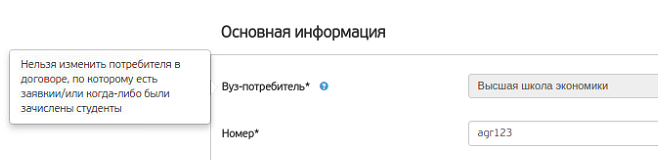
\includegraphics[width=1\linewidth]{consumer_help.png}}
	\caption{Подсказка о невозможности изменения значения поля вуз"=потребитель}
	\label{agreement:consumer_help}
\end{figure}
	\item \textbf{Номер.} Номер договора;
	\item \textbf{Дата начала договора};
	\item \textbf{Дата окончания договора};
	\item \textbf{Контактное лицо.} Контактное лицо со стороны вуза"=потребителя для связи по данному договору;
	\item \textbf{Контакты контактного лица.} Контакты (e"=mail, номер телефона, др.) контактного лица со стороны вуза"=потребителя для связи по данному договору;
	\item \textbf{Статус.} Статус договора принимает одно из трех возможных значений: \quotes{Черновик},  \quotes{Действует},  \quotes{Не действует}. Создание заявок на зачисление на стороне потребителя возможно только по действующему договору. Договоры, имеющие статус  \quotes{Черновик} и \quotes{Не действует} не показываются потребителям в соответствующем разделе \quotes{Договоры на получение услуг};
	\item \textbf{Примечание}. Любое примечание к договору;
	\item \textbf{Курсы.} Курсы, которые добавлены к данному договору.
\end{itemize}

\subsubsection{Поля и ошибки}
В форме представлено несколько типов полей:
	\begin{itemize}
		\item \textbf{Обязательные поля} отмечены символом \quotes{*}, если такое поле оставить не заполненным "--- появляется сообщение о необходимости его заполнения и блокируется кнопка сохранения изменений (см. рис.~\ref{agreement:edit_required}).
		
		\begin{figure}[H]
		\center{\includegraphics[width=1\linewidth]{edit_required.png}}
		\caption{Обработка заполнения обязательных полей}
		\label{agreement:edit_required}
		\end{figure}	
		
		\item \textbf{Даты начала и окончания договора.} "--- виджет выбора даты, подробно описанный в подразделе~\ref{widget:date_time_picker};
	\end{itemize} 
		
\subsubsection{Курсы} Данный элемент формы представляет собой подраздел, в котором происходит редактирование курсов, на которые заключается договор. Каждый курс представлен в этой области строкой-формой, которая включает в себя элементы:
		\begin{itemize}
			\item \textbf{Название курса.} Выбор происходит из выпадающего списка, среди вариантов все курсы данного вуза, кроме уже добавленных к договору.
			\item \textbf{Количество студентов.} Максимальное количество студентов, которое планируется зачислить по данному курсу в рамках договора, при превышении этого количества на этапе принятия/отклонения заявок на зачисление администратор вуза, будет получать предупреждения, может быть не заполнено, тогда ограничения нет. Если это поле заполнено, то в соответствующей строке-форме должно быть заполнено и поле \quotes{Название курса}, в противном случае при сохранении формы будет выведена ошибка, подробнее об этом ниже.
			\item \textbf{Зачислено.} Фактическое количество зачисленных студентов по данному курсу в рамках договора на текущий момент.
		\end{itemize}
		Внешний вид области редактирования курсов представлен на рисунке~\ref{agreement:edit_course}.
		\begin{figure}[H]
			\center{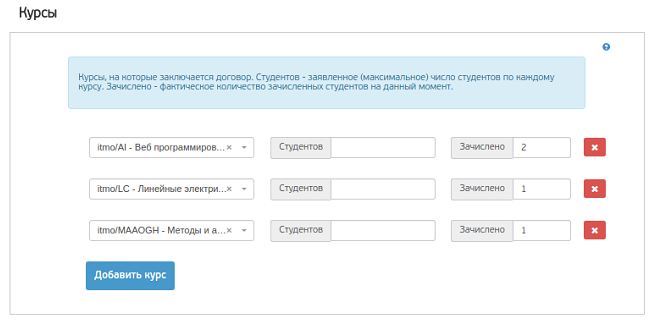
\includegraphics[width=1\linewidth]{edit_course.png}}
			\caption{Внешний вид области редактирования курсов}
			\label{agreement:edit_course}
		\end{figure}	

Механизм работы с договорами предполагает несколько сценариев:
\begin{itemize}
	\item При создании/редактировании договора указываются курсы, на которые заключается договор. Курс, который добавлен в форме создания/редактирования договора, называется \quotes{зафиксированным}. После сохранения договора с добавленными курсами подавать заявки, производить зачисления по этому договору можно только на зафиксированные курсы. Курс в договоре, по которому есть заявки и/или когда-либо были зачислены студенты с указанием этого договора называется \quotes{активным}, в противном случае \quotes{неактивным}.
	\item При создании/редактирования договора не указываются никакие курсы. После сохранения договора с пустым блоком курсов подавать заявки/производить зачисления по этому договору можно на любые курсы данного вуза.  Курс в договоре, по которому есть заявки и/или когда-либо были зачислены студенты с указанием этого договора называется \quotes{активным}, в противном случае \quotes{неактивным}.
\end{itemize}

Курс называется \quotes{связанным с договором}, если он активный и/или зафиксированный. \\
Если на редактирование открыт договор, среди связанных курсов которого есть активные, но не зафиксированные (был создан договор с пустым блоком курсов, далее были поданы заявки/произведены зачисления на какие-либо курсы по этому договору), то в блоке курсов будет видна кнопка \quotes{Зафиксировать курсы} (см. рис.~\ref{agreement:edit_course_fix_button}), подсказка о предназначении кнопки будет выведена в блоке подсказок над формами курсов по нажатию на иконку \vcenteredinclude[width=0.05\linewidth]{help_icon.png} .
		
		\begin{figure}[H]
			\center{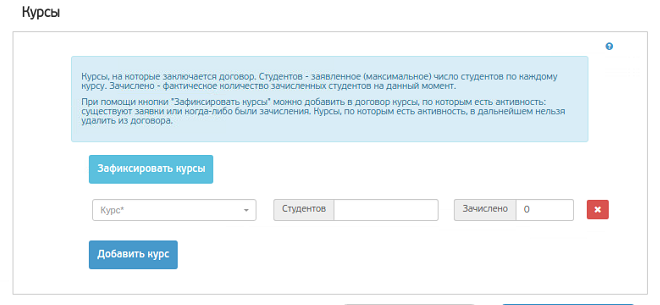
\includegraphics[width=1\linewidth]{edit_course_fix_button.png}}
			\caption{Кнопка \quotes{Зафиксировать курсы}}
			\label{agreement:edit_course_fix_button}
		\end{figure}	

По нажатию кнопки \quotes{Зафиксировать курсы} активные курсы будут добавлены к договору, сама кнопка будет скрыта, информация о ней исчезнет из блока подсказок (см. рис.~\ref{agreement:edit_course_fixed}). В дальнейшем, после сохранения из договора нельзя будет удалить активные курсы, подробнее об этом см. ниже.
		
		\begin{figure}[H]
		\center{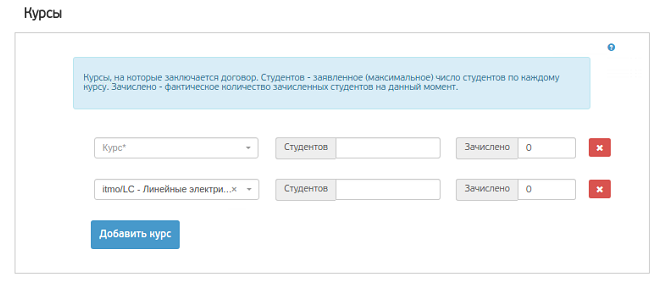
\includegraphics[width=1\linewidth]{edit_course_fixed.png}}
		\caption{Зафиксированные курсы}
		\label{agreement:edit_course_fixed}
		\end{figure}	

	Для того, чтобы добавить курс к договору необходимо нажать на кнопку \quotes{Добавить}(см. рис.~\ref{agreement:edit_course_add}). В появившейся строке можно выбрать курс из числа курсов, предоставляемых данным вузом, которые еще не добавлены к данному договору. Один и тот же курс может быть добавлен к договору не больше одного раза. Подробная информация о работе с полями, содержащими виджет выпадающего списка с автодополнением доступна в разделе~\ref{widget:autocomplete}. Если заполнено поле \quotes{Студентов}, то поле \quotes{Курс} в этой же строке-форме является обязательным для заполнения, если попробовать сохранить формы с добавленной, но не заполненной строкой курса, появится сообщение об ошибке (см. рис.~\ref{agreement:edit_course_required}). Сохранение при наличии в блоке курсов любого количества пустых форм возможно, такие формы буду отброшены.
		
		\begin{figure}[H]
		\center{\includegraphics[width=1\linewidth]{edit_course_add.png}}
		\caption{Добавление курса к договору}
		\label{agreement:edit_course_add}
		\end{figure}	
		
		\begin{figure}[H]
		\center{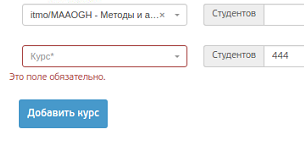
\includegraphics[height=3cm]{edit_course_required.png}}
		\caption{Ошибка сохранения формы с незаполненным полем курса при заполненном поле \quotes{Студентов}}
		\label{agreement:edit_course_required}
		\end{figure}	
		
	Для того, чтобы совершить попытку удаления курса из договора необходимо нажать на иконку \vcenteredinclude[width=0.07\linewidth]{edit_course_delete.png} в соответствующей строке-форме. \\
Возможны следующие сценарии:
\begin{itemize}
	\item если курс неактивный, он будет исключен из блока курсов и удален из добавленных к договору курсов, после сохранения формы редактирования договора;
	\item если курс активный (но нему имеются заявки или когда-либо были зачислены студенты с указанием данного договора), то удалить его из договора нельзя. Пользователь увидит модальное окно с информацией о причинах, по которым нельзя удалить курс. (см. рис.~\ref{agreement:edit_course_warn}).
	\begin{figure}[H]
		\center{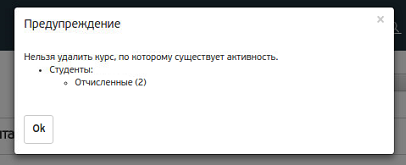
\includegraphics[width=1\linewidth]{edit_course_warn.png}}
		\caption{Модальное окно при невозможности сохранения курса}
		\label{agreement:edit_course_warn}
	\end{figure}	
Если нажать кнопку \quotes{Ок}, "Х" в модальном окне  или кликнуть за его пределы, то модальное окно закроется, пользователь останется в разделе \quotes{Редактирование договора}
\end{itemize}


Если указанное значение количества студентов в договоре меньше, чем количество уже зачисленных студентов по этому договору, то
при сохранении формы появится окно с предупреждением (см. рис.~\ref{agreement:edit_course_warn_number}).

		\begin{figure}[H]
		\center{\includegraphics[width=1\linewidth]{edit_course_warn_number.png}}
		\caption{Предупреждении о превышении максимального количества студентов}
		\label{agreement:edit_course_warn_number}
		\end{figure}
		
Если нажать \quotes{Ок} "--- форма будет сохранена, в случае нажатия кнопки \quotes{Отмена} или клику за пределы окна с предупреждением, процесс сохранения изменений будет остановлен, поле, в котором произошло превышение, будет подсвечено красным (см рис.~\ref{agreement:edit_course_warn_cancel}).	

		\begin{figure}[H]
		\center{\includegraphics[width=1\linewidth]{edit_course_warn_cancel.png}}
		\caption{Предупреждении о превышении максимального количества студентов}
		\label{agreement:edit_course_warn_cancel}
		\end{figure}

 	
\subsubsection{Элементы управления}
Управление внесенными изменениями осуществляется с помощью кнопок расположенных внизу страницы (см. рис.~\ref{agreement:edit_buttons}).
		\begin{figure}[H]
		\center{
\includegraphics[width=1\linewidth]{edit_buttons.png}}
		\caption{Элементы управления подраздела \quotes{Редактирование договора}}
		\label{agreement:edit_buttons}
		\end{figure}	
		
При нажатии \quotes{Сохранить} осуществляется попытка сохранения формы. 
Если форма заполнена корректно, то внесенные изменения сохраняются, а пользователь перенаправляется в раздел \quotes{Просмотр подробной информации о договоре}.
Если имеются ошибки "--- отображаются сообщения об ошибках, осуществляется прокрутка к месту первой ошибки. 

При нажатии кнопки \quotes{Отмена} все изменения теряются, пользователь перенаправляется на предыдущую страницу.


\subsection{Добавить договор}
Подраздел позволяет пользователям роли \quotes{Администратор вуза} создать договор на предоставление услуг вузу"=потребителю.\\

Переход в подраздел осуществляется по выбору соответствующего пункта вспомогательного меню, расположенного на левой панели.\\

Форма создания, ее состав, возможные действия и реакции аналогичны описанным в разделе~\ref{agreement:edit_section}, за исключение нескольких отличий в блоке \quotes{Курсы}:\\
Так как по еще не созданному договору не может быть никакой активности (заявок или зачислений на курсы с указанием этого договора), то в строках-формах блока отсутствует графа \quotes{Зачислено}, расположенный над строкам-формами содержит минимальную информацию о значении полей (см. рис.~\ref{agreement:create_course}).
		\begin{figure}[H]
		\center{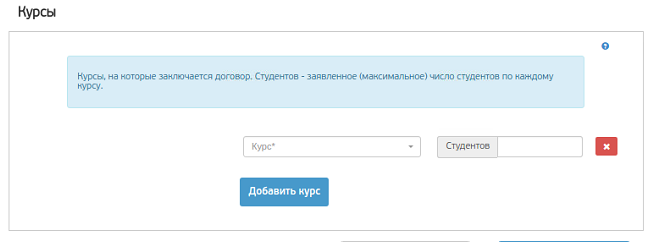
\includegraphics[width=1\linewidth]{create_course.png}}
		\caption{Блок курсов при создании договора}
		\label{agreement:create_course}
		\end{figure}	


\subsection{Платежи}
Данный подраздел предоставляет информацию о платежах.\\

Переход в подраздел осуществляется по выбору соответствующего пункта вспомогательного меню, расположенного на левой панели.\\

Информация о платежах представлена в виде таблицы, каждая строка которой соответствует конкретному платежу. 
Таблица имеет следующие колонки:
\begin{itemize}
	\item \textbf{Дата создания.} Дата создания платежа
	\item \textbf{Студент.} Студент, который осуществляет платеж.
	\item \textbf{Сумма заказа.} Сумма, на которую осуществляется платеж.
	\item \textbf{Номер заказа.}
	\item \textbf{Статус платежа}. Возможны следующие значения: \quotes{Processed}, \quotes{Success}, \quotes{Fail}.
	\item \textbf{Дата платежа.} Дата, соответствующая моменту, когда платеж произведен.
\end{itemize}

Внешний вид раздела представлен на рисунке~\ref{agreement:table_payments}.
		\begin{figure}[H]
		\center{\includegraphics[width=1\linewidth]{table_payments.png}}
		\caption{Внешний вид подраздела \quotes{Платежи}}
		\label{agreement:table_payments}
		\end{figure}	
		
\subsubsection{Элементы управления}
Элементы управления табличными представления описаны в подразделе~\ref{sec:datatables}. Вид формы фильтрации приведён на рисунке~\ref{agreement:payments_filter_form}
\begin{figure}[H]
	\center{\includegraphics[height=10.5cm]{payments_filter_form.png}}
	\caption{Вид формы фильтрации для подраздела \quotes{Платежи}}
	\label{agreement:payments_filter_form}
\end{figure}

Можно фильтровать список по следующим параметрам:
\begin{itemize}
	\item Диапазон дат создания "--- виджеты выбора даты и времени 
	(описание виджета см. в подразделе~\ref{widget:date_time_picker});
	\item Пользователь "--- виджет выпадающего списка с автодополнением с возможностью множественного выбора 
	(описание виджета см. в подразделе~\ref{widget:autocomplete_with_multiselect});
	\item Диапазон суммы заказа "--- числовое поле.
	\item Номер заказа "--- текстовое поле.
	\item Статус "--- виджет выпадающего списка с автодополнением с возможностью множественного выбора 
	(описание виджета см. в подразделе~\ref{widget:autocomplete_with_multiselect});
	\item Диапазон дат платежа "--- виджеты выбора даты и времени.
\end{itemize}


\subsection{Заявки на зачисление студентов}

Заявки на зачисление "--- это табличное представление заявок на зачисление студентов, 
полученных данным вузом в качестве вуза-разработчика. 
Элементы управления табличными представления описаны в подразделе~\ref{sec:datatables}.
Внешний вид списка представлен на рис.~\ref{img:agreement:enroll_req_list}. 

\begin{figure}[H]
	\center{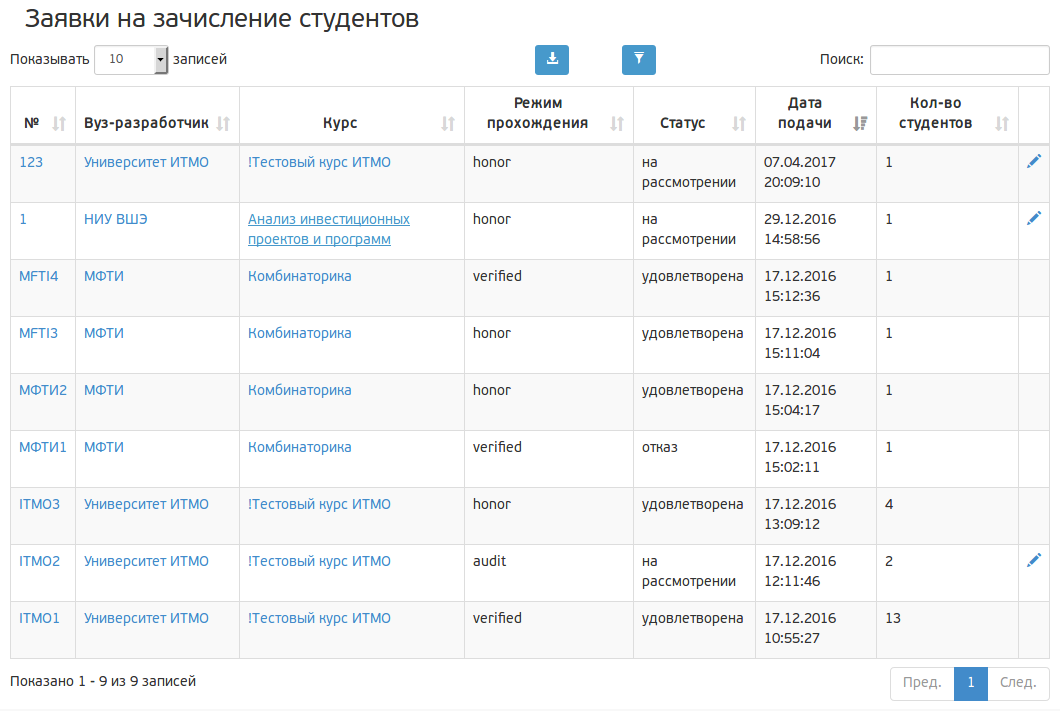
\includegraphics[width=1\linewidth]{enroll_req_list}}
	\caption{Список заявок на зачисление}
	\label{img:agreement:enroll_req_list}
\end{figure}

Таблица содержит следующие столбцы:
\begin{itemize}
	\item \textbf{Номер заявки.};
	\item \textbf{Вуз-потребитель.} Вуз, который подал заявку;
	\item \textbf{Курс.} Курс на который подана заявка;
	\item \textbf{Режим прохождения.};
	\item \textbf{Статус.} Текущий статус заявки;
	\item \textbf{Дата подачи.};
	\item \textbf{Количество студентов.} Сколько студентов указано в заявке.
\end{itemize}

 Номер заявки в таблице является ссылкой на страницу просмотра подробной информации о заявке, 
описанной в подразделе~\ref{sec:enroll_req_detail}.

Внешний вид диалога фильтрации списка заявок представлен на рис.~\ref{img:agreement:enroll_req_list_filter}.
Можно фильтровать список по следующим параметрам:
\begin{itemize}
	\item Вуз-потребитель "--- виджет выпадающего списка с автодополнением с возможностью множественного выбора 
	(описание виджета см. в подразделе~\ref{widget:autocomplete_with_multiselect});
	\item Курс "--- виджет выпадающего списка с автодополнением с возможностью множественного выбора 
	(описание виджета см. в подразделе~\ref{widget:autocomplete_with_multiselect});
	\item Режим прохождения "--- виджет выпадающего списка с автодополнением с возможностью множественного выбора 
	(описание виджета см. в подразделе~\ref{widget:autocomplete_with_multiselect});
	\item Статус "--- виджет выпадающего списка с автодополнением с возможностью множественного выбора 
	(описание виджета см. в подразделе~\ref{widget:autocomplete_with_multiselect});
	\item Диапазон дат подачи "--- виджеты выбора даты и времени 
	(описание виджета см. в подразделе~\ref{widget:date_time_picker});
	\item Диапазон количества студентов в заявке "--- числовое поле.
\end{itemize}

\begin{figure}[H]
	\center{\includegraphics[height=9.1cm]{enroll_req_list_filter}}
	\caption{Диалог фильтрации списка заявок на зачисление}
	\label{img:agreement:enroll_req_list_filter}
\end{figure}

\subsection{Заявки на изменение режима прохождения сессии курса}

Заявки на изменение режима прохождения сессии курса -- это табличное представление заявок на изменение 
режима прохождения сессии курса, полученных данным вузом в качестве вуза-разработчика. 
Элементы управления табличными представления описаны в подразделе~\ref{sec:datatables}.
Внешний вид списка представлен на рис.~\ref{img:agreement:change_mode_req_list}. 

\begin{figure}[H]
	\center{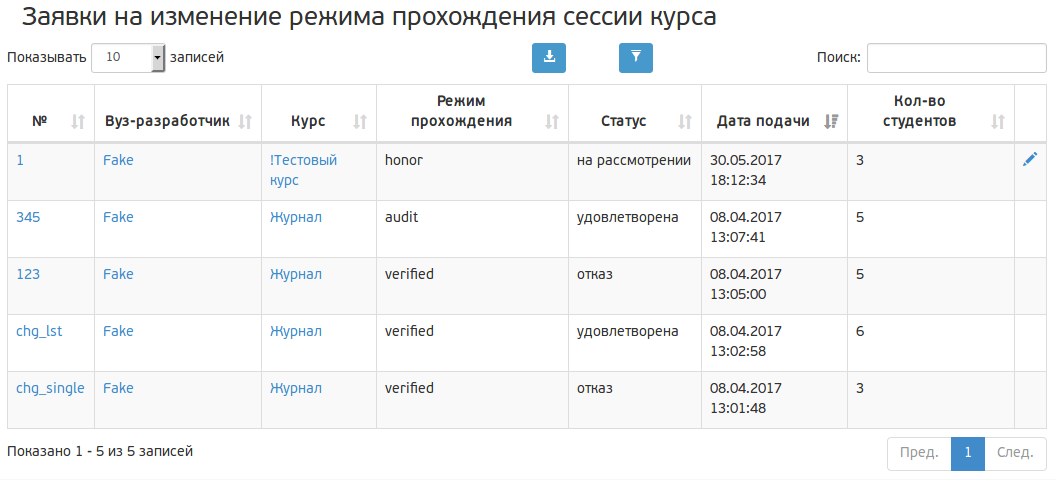
\includegraphics[width=1\linewidth]{change_mode_req_list}}
	\caption{Список заявок на изменение режима прохождения сессии курса}
	\label{img:agreement:change_mode_req_list}
\end{figure}

Таблица содержит следующие столбцы:
\begin{itemize}
	\item \textbf{Номер заявки.};
	\item \textbf{Вуз-потребитель.} Вуз, который подал заявку;
	\item \textbf{Курс.} Курс на который подана заявка;
	\item \textbf{Режим прохождения.};
	\item \textbf{Статус.} Текущий статус заявки;
	\item \textbf{Дата подачи.};
	\item \textbf{Количество студентов.} Сколько студентов указано в заявке.
\end{itemize}

Номер заявки в таблице является ссылкой на страницу просмотра подробной информации о заявке, 
описанной в подразделе~\ref{sec:change_mode_req_detail}.

Внешний вид диалога фильтрации списка заявок представлен на рис.~\ref{img:agreement:change_mode_req_list_filter}.
Можно фильтровать список по следующим параметрам:
\begin{itemize}
	\item Вуз-потребитель "--- виджет выпадающего списка с автодополнением с возможностью множественного выбора 
	(см. подраздел~\ref{widget:autocomplete_with_multiselect});
	\item Курс "--- виджет выпадающего списка с автодополнением с возможностью множественного выбора 
	(см. подраздел~\ref{widget:autocomplete_with_multiselect});
	\item Режим прохождения "--- виджет выпадающего списка с автодополнением с возможностью множественного выбора 
	(см. подраздел~\ref{widget:autocomplete_with_multiselect});
	\item Статус "--- виджет выпадающего списка с автодополнением с возможностью множественного выбора 
	(см. подраздел~\ref{widget:autocomplete_with_multiselect});
	\item Диапазон дат подачи "--- виджеты выбора даты и времени 
	(см. подраздел~\ref{widget:date_time_picker});
	\item Диапазон количества студентов в заявке "--- числовое поле.
\end{itemize}

\begin{figure}[H]
	\center{\includegraphics[height=9cm]{enroll_req_list_filter}}
	\caption{Диалог фильтрации списка заявок на изменение режима прохождения сессии курса}
	\label{img:agreement:change_mode_req_list_filter}
\end{figure}

